\section{System Implementation}
\subsection{System login module implementation}
\subsubsection{Flow Chart}
The Flow chart is shown as Figure \ref{fig:p6}
\begin{figure}[H]
    \centering
    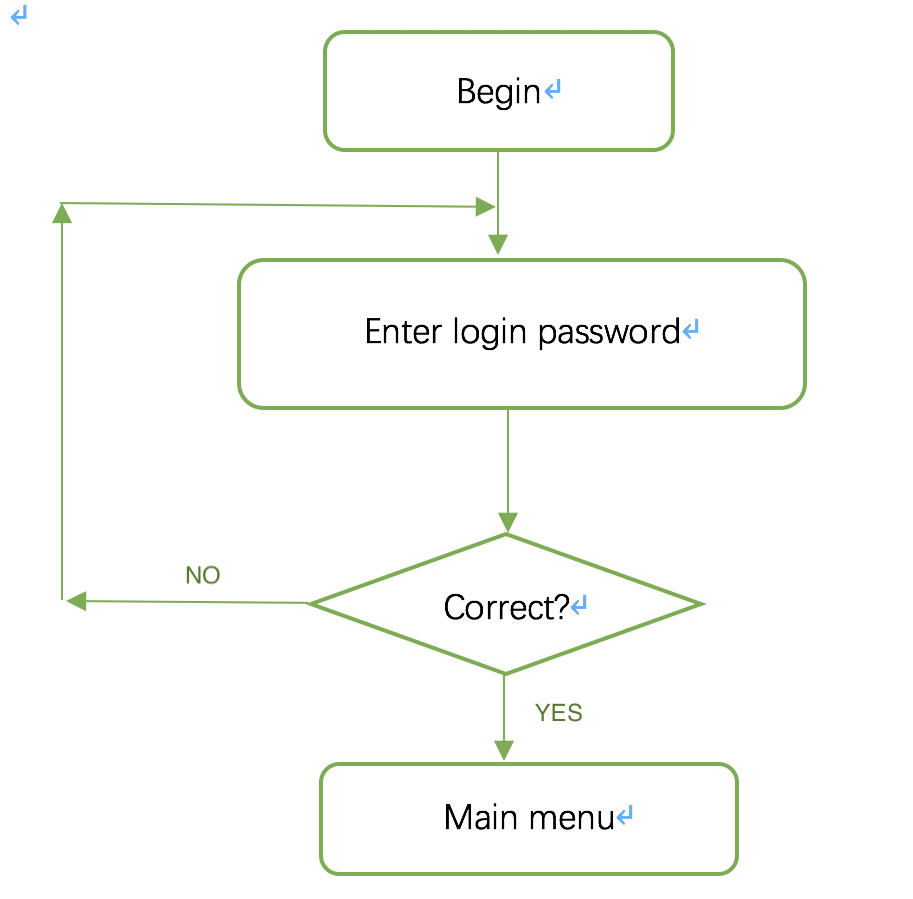
\includegraphics[width=\textwidth]{6.png}
    \caption{Flow Chart}
    \label{fig:p6}
\end{figure}
\subsubsection{User Interface}
The User Interface is shown as Figure \ref{fig:p7}
\begin{figure}[H]
    \centering
    \includegraphics[width=\textwidth]{7.png}
    \caption{Interface}
    \label{fig:p7}
\end{figure}
Relative functions:

\begin{enumerate}
    \item As we can see, this interface consists of two input boxes and two buttons. After the user enters his own information into the corresponding input box, click the login button to submit the data in the input box. 
    \begin{itemize}
        \item If the user enters the correct information, the system will let the client jump to the main page. 
        \item If there is any inconsistency, the corresponding error message is given.
    \end{itemize}
    \item Input: user name and password.
    \item Relevant processing: 
        \begin{itemize}
            \item First, the validity of the user name and password is checked through the check of the foreground JS, mainly to prevent the user from entering illegal characters. 
            \item After the verification of the front desk JS, the system will pass the user submitted data the day after tomorrow, let the server to check whether the user name exists or the password is correct.
        \end{itemize}
    \item Output: 
    \begin{itemize}
        \item If the user login is successful, he enters the user's system home page, and displays the related menu interface and provides the corresponding role operation according to the user's related type utype.
        \item If the login is unsuccessful, an error information page is displayed.
    \end{itemize} 
\end{enumerate}
\subsection{The realization of the main interface}
\subsubsection{Administrator main interface}
\label{sec:admin}
The administrator's main interface is expressed in the form of a menu, as shown in figure \ref{fig:p8}.
\begin{figure}[H]
    \centering
    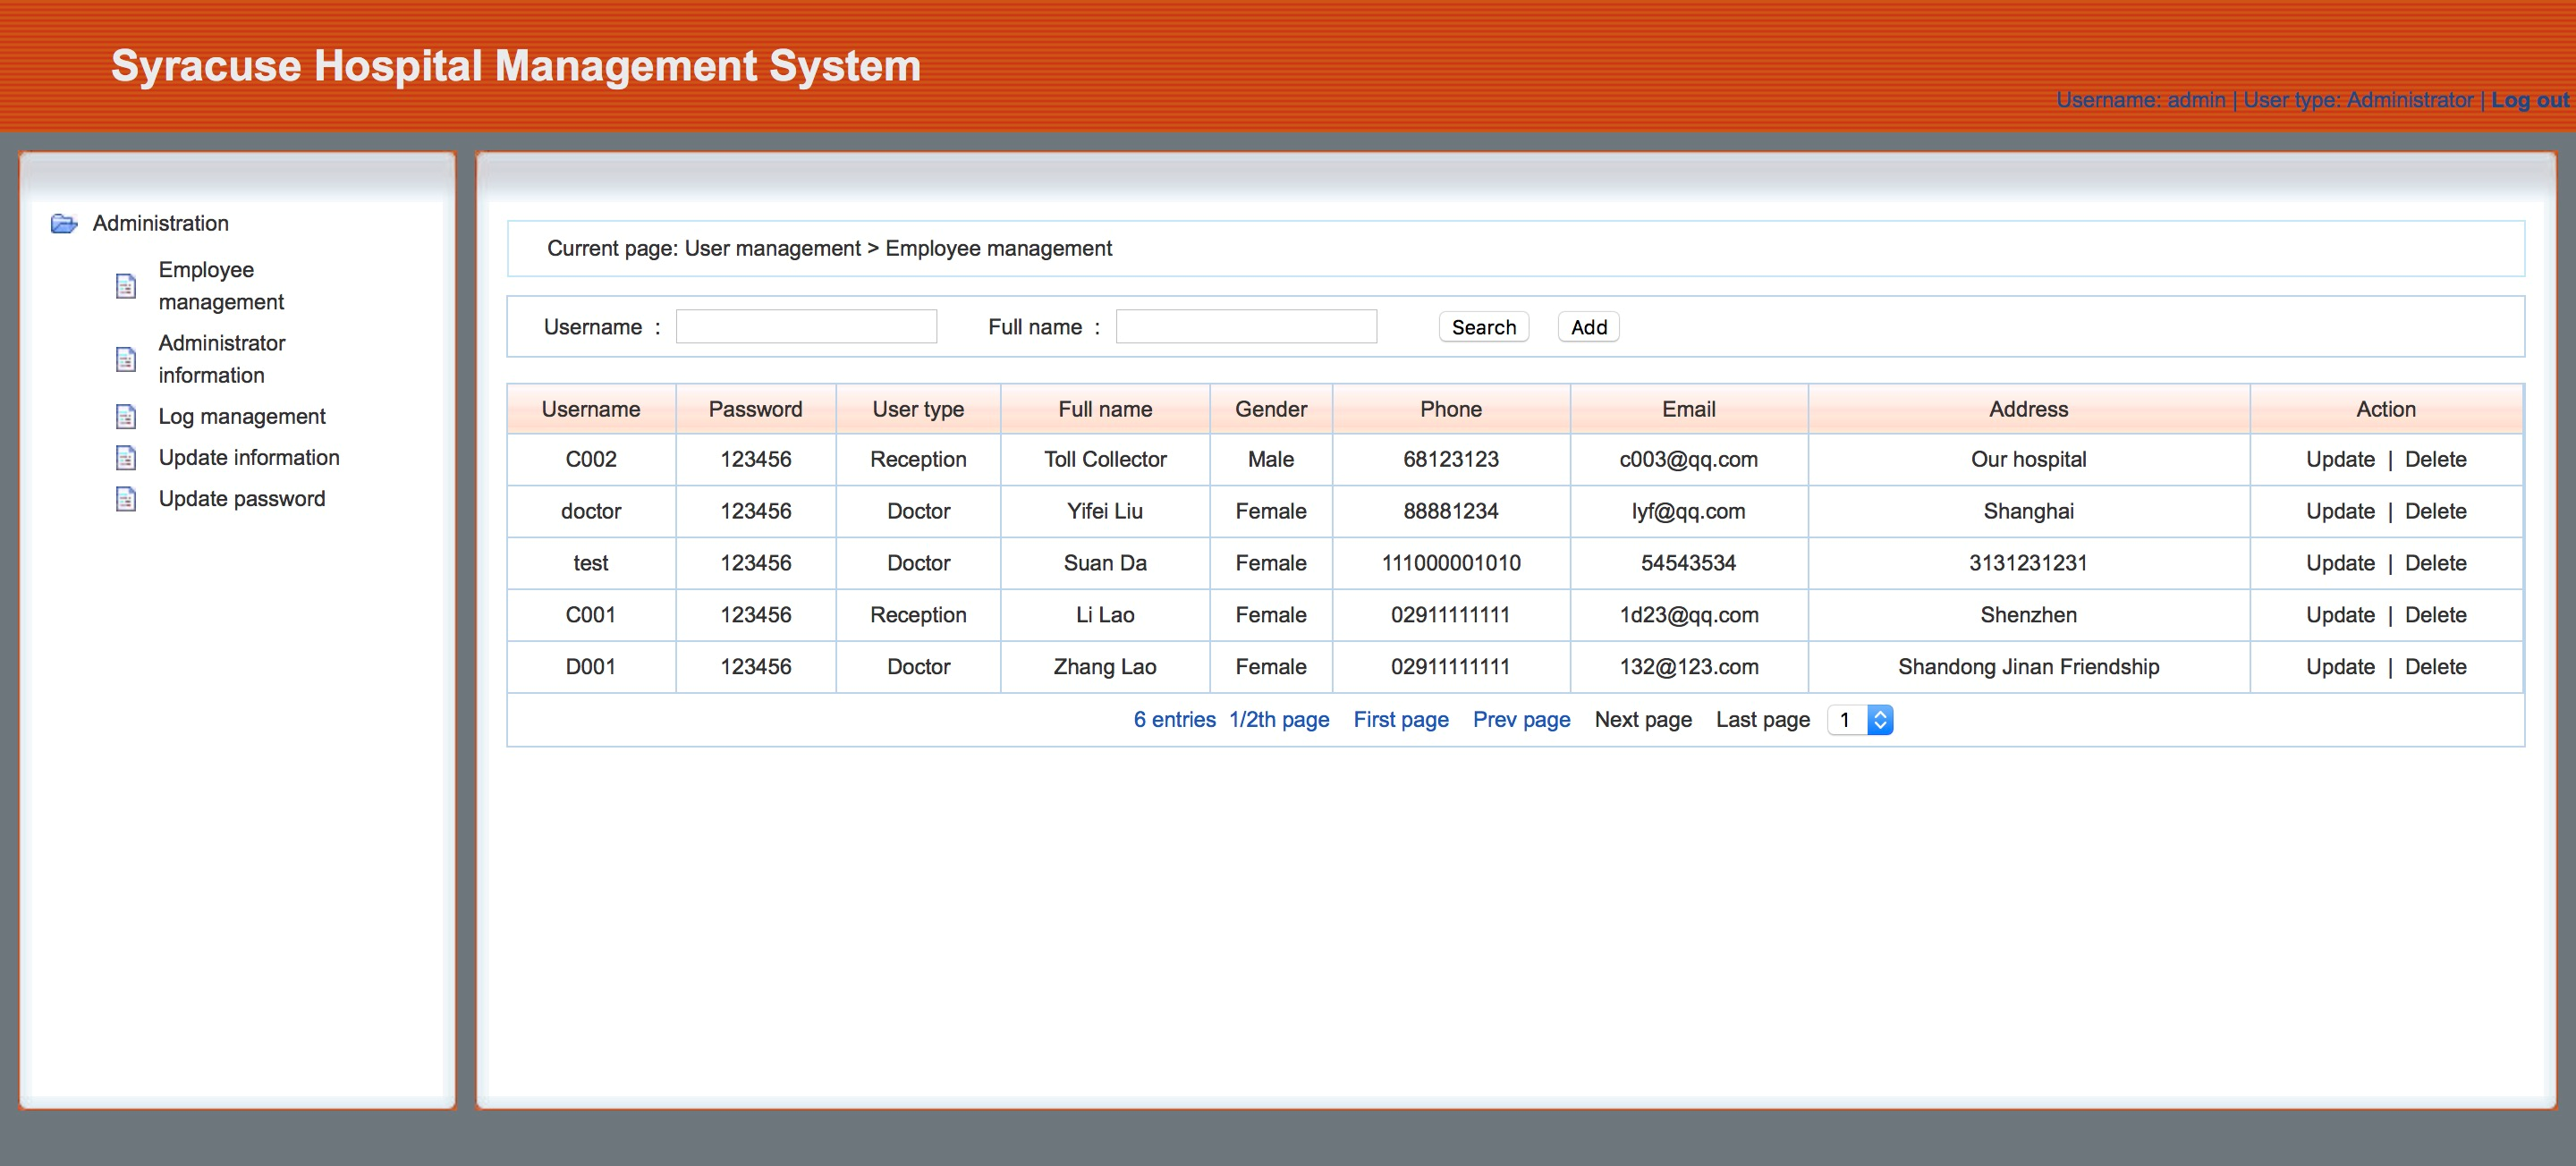
\includegraphics[width=\textwidth]{8.png}
    \caption{Administrator interface}
    \label{fig:p8}
\end{figure}
The main functions are as follows:
\begin{enumerate}
    \item Staff management: The management of other roles except the system administrator, including the addition, modification, and deletion of their passwords and other detailed information, can also be performed on the user based on the user name and name.
    \item  Administrator user information: In addition to managing general employee information, administrators can also manage administrator related information, such as adding administrators.
    \item Log Management: Administrators can view and search the log information in the system, including searching according to the operator, and searching according to the operation record number. In this system, the log information is used in related operations, the system automatically in the database The relevant log information is inserted, where the log information is mainly divided into two types, one is an ordinary login operation, and the other is a new modification operation of the medical record, and the log records the operator, operation time and other related information.
    \item Modify personal information: Administrators can make some modifications to their own details.
    \item Modify login password: According to the existing password administrator, you can update your own password.
\end{enumerate}
\subsubsection{Reception main interface}
The window staff main interface is represented by a menu, as shown in Figure \ref{fig:p9}.
\begin{figure}[H]
    \centering
    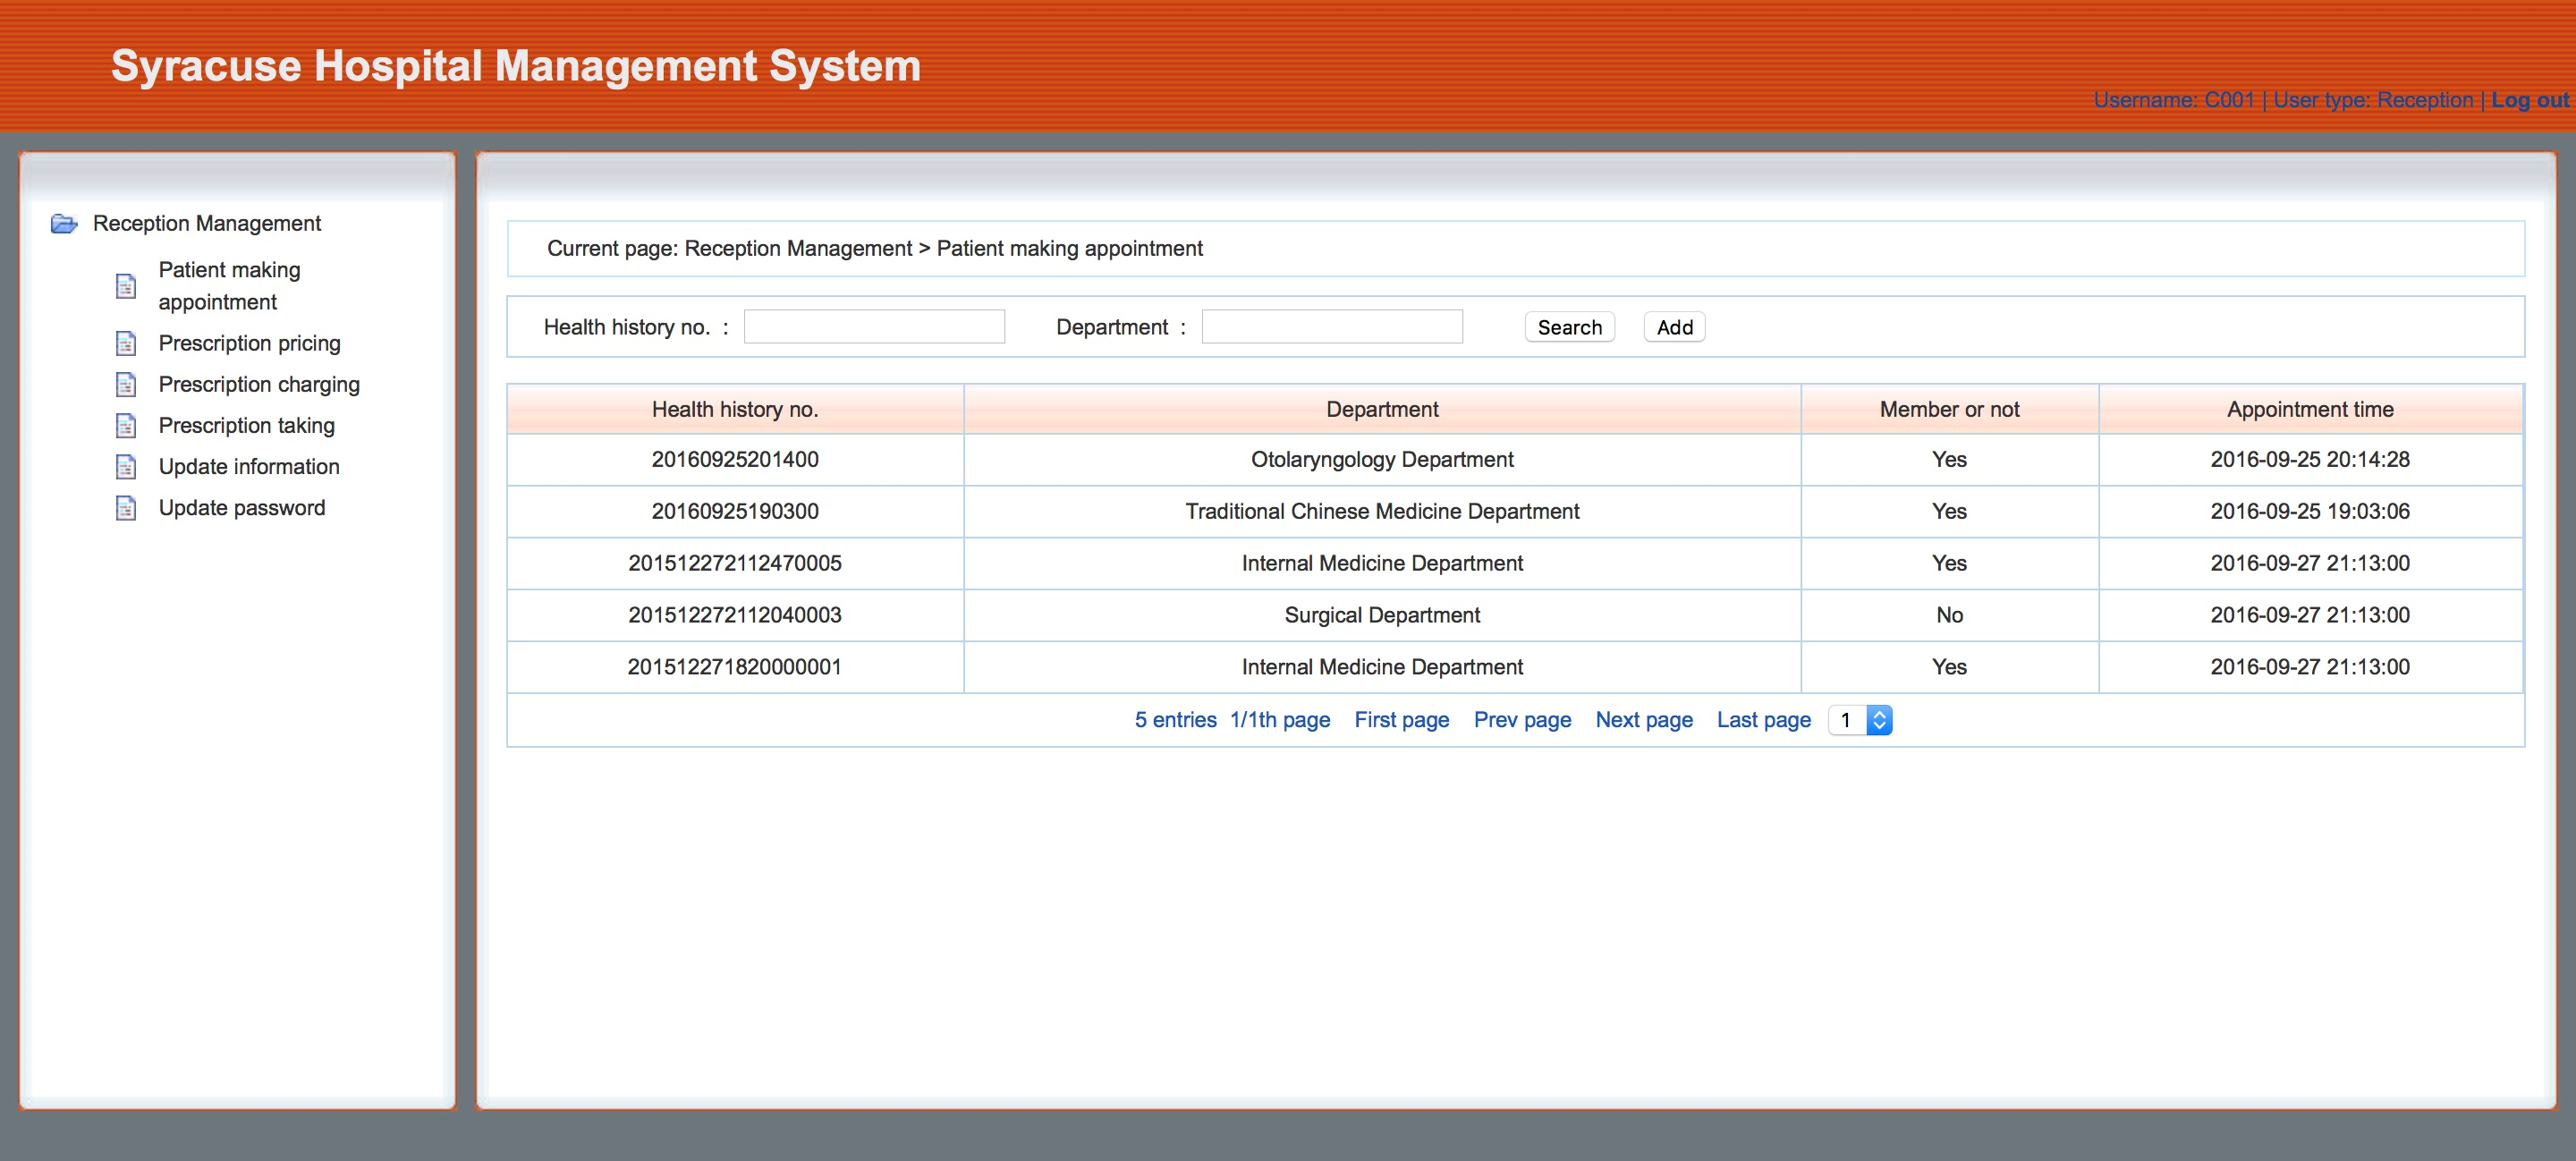
\includegraphics[width=\textwidth]{9.png}
    \caption{Reception interface}
    \label{fig:p9}
\end{figure}
The main functions are as follows:
\begin{enumerate}
    \item Patient Registration: After the patient arrives at the hospital, the patient is registered at the window. The window personnel will register the relevant information and inform the patient of the patient's medical record number. The patient can find the doctor in the relevant department with the patient's medical record number.
    \item Prescription markup: When the doctor fills out the medical record and opens the benefits, the patient comes to the window with a good case for the prescription price.
    \item Prescription payment: After the prescription price is completed, the patient will perform the payment operation and calculate different according to whether the patient has medical insurance.
    \item Prescription medicine: After the patient completes the doctor's fee payment operation, he can go to the window to take medicine. However, if the patient has not paid, the window person cannot find the patient's medicine information in the medicine picking list.
    \item Modify Personal Information: The window personnel can modify their own details after logging in to the system.
    \item Modify login password: After logging into the system, the window personnel can update their own password based on the existing password.
\end{enumerate}
\subsubsection{Doctor's main interface}
The doctor's main interface is represented by a menu, as shown in Figure \ref{fig:p10}.
\begin{figure}[H]
    \centering
    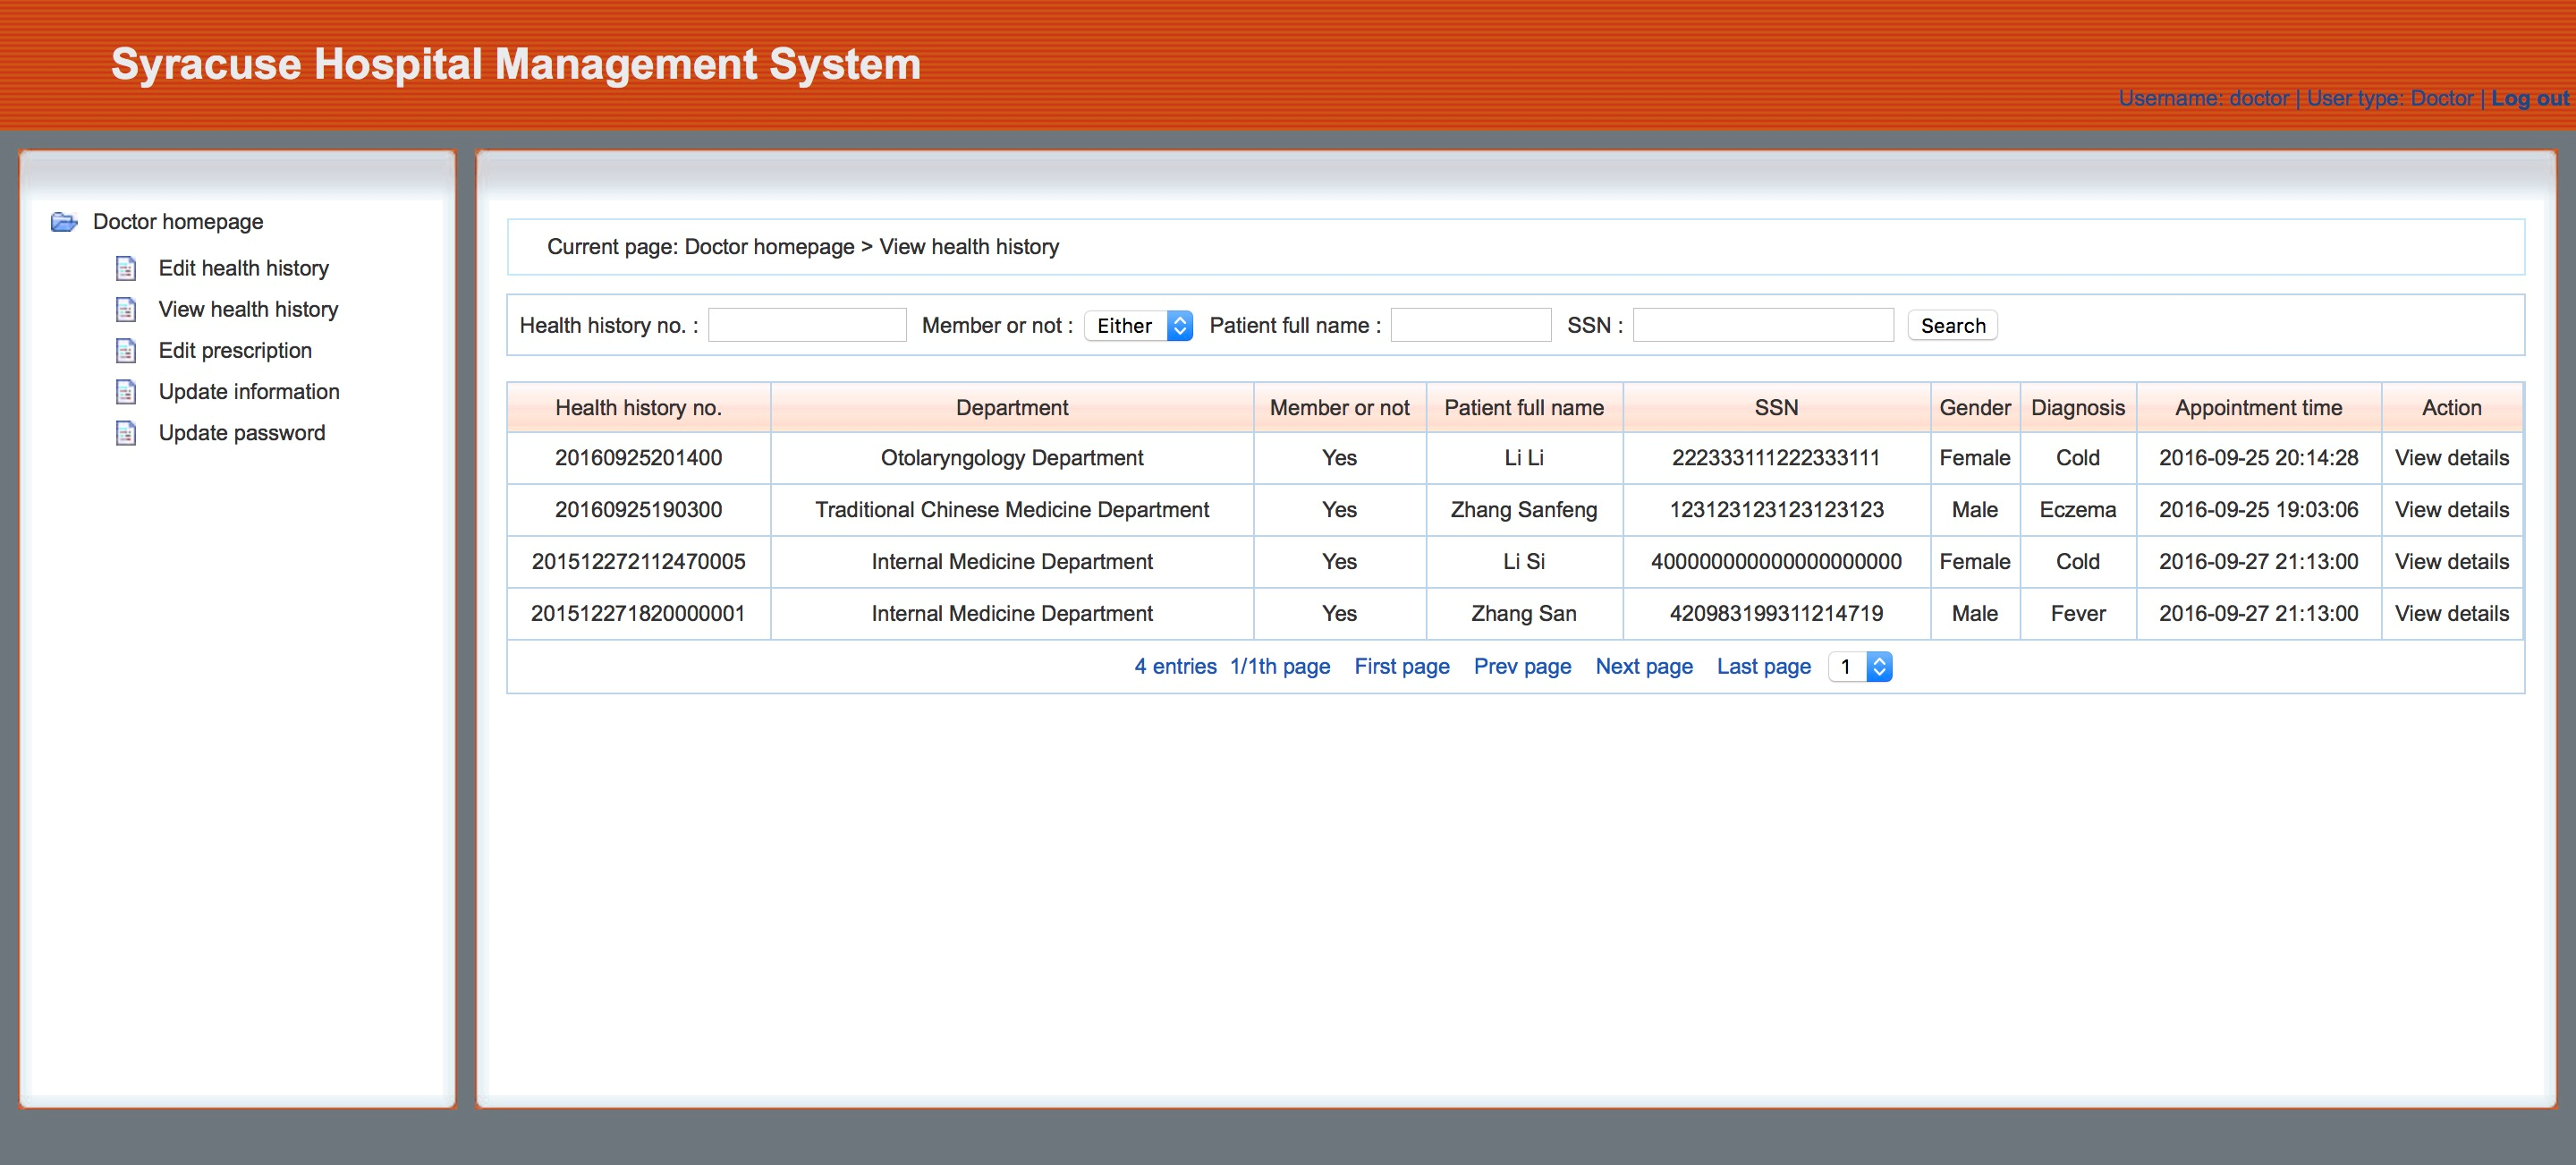
\includegraphics[width=\textwidth]{10.png}
    \caption{Doctor interface}
    \label{fig:p10}
\end{figure}
The main functions are as follows:
\begin{enumerate}
    \item The patient: The doctor can find the patient's medical record according to the patient's medical record number and fill in the relevant information of the medical record.
    \item medical records view: doctors can search for relevant medical records based on different information of patients, including patient's name, ID number, medical record number and other relevant information.
    \item Prescription management: After the doctor fills out the patient's medical records, he can prescribe drugs to the patient. In this interface, the doctor can add prescription information, view the prescription information and find relevant prescriptions based on the medical record number and drug name, modify and delete. Related prescription information.
    \item modify personal information: After the doctor logs on the system can modify their own detailed personal information.
    \item modify the login password: Like other users, doctors can also follow their own password to keep up with their own password.
\end{enumerate}

\subsubsection{Warehouse keeper home screen}
The drug administrator is represented by a menu, as shown in Figure \ref{fig:p11}.
\begin{figure}[H]
    \centering
    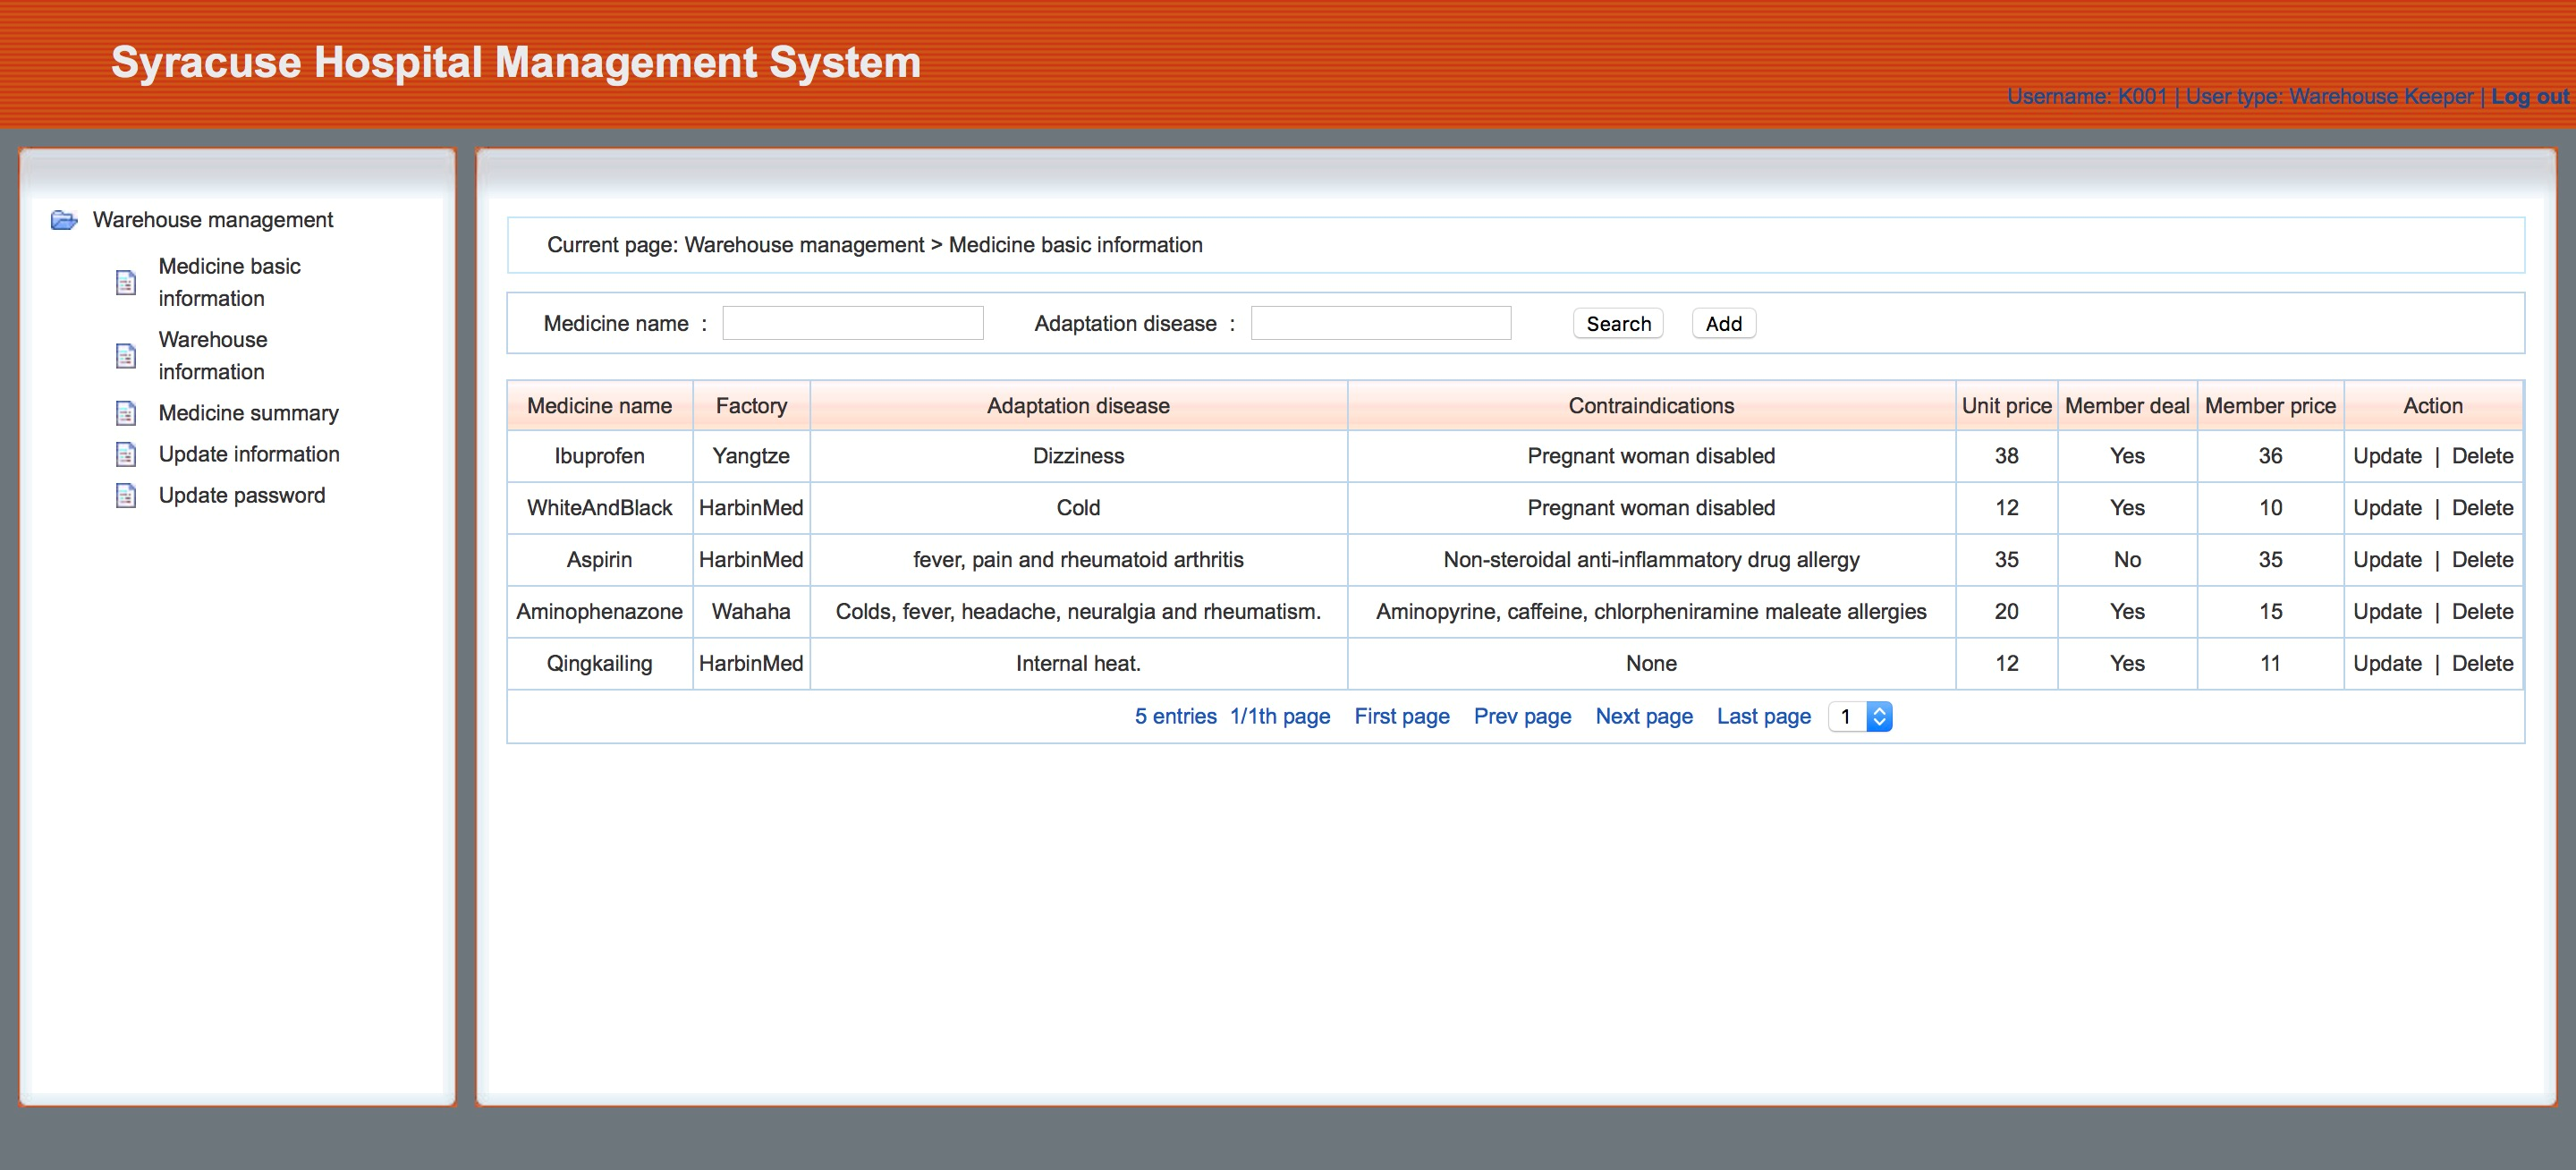
\includegraphics[width=\textwidth]{11.png}
    \caption{Warehouse keeper interface}
    \label{fig:p11}
\end{figure}
The main functions are as follows:
\begin{enumerate}
    \item Drug basic information management: After the warehouse administrator logs in the system, he can add new drugs or modify existing drug information through the form, and can also query the corresponding drugs based on the drug name and applicable symptoms.
    \item Management of drug storage information: The library management personnel can add information on the storage of drugs, including information on time of storage, batch number of storage, etc., and can modify the relevant information of storage, and can also check according to the drug name and storage time. Related storage information.
    \item Drug inventory: The warehouse personnel can view the inventory information of the drug, including the inbound quantity, current inventory, total purchase amount and total sales, and purchase the goods according to the current inventory and sales.
    \item  modify personal information: inventory personnel can modify their own details after logging in the system.
    \item modify the login password: inventory personnel can log in to the system can update their own password based on the existing password.
\end{enumerate}

